\documentclass[unicode,11pt,a4paper,oneside,numbers=endperiod,openany]{scrartcl}
\newcommand\tab[1][0.5cm]{\hspace*{#1}}
\usepackage{array}
\usepackage{multirow}
\usepackage{graphicx}
\usepackage[utf8]{inputenc}
\usepackage{listings}
\usepackage{xcolor}
\usepackage{seqsplit}
\usepackage{float}
\usepackage{booktabs}
\usepackage{subcaption}
\usepackage{adjustbox}
\usepackage{listings}
%New colors defined below
\definecolor{codegreen}{rgb}{0,0.6,0}
\definecolor{codegray}{rgb}{0.5,0.5,0.5}
\definecolor{codepurple}{rgb}{0.58,0,0.82}
\definecolor{backcolour}{rgb}{0.98,0.98,0.98}
%Code listing style named "mystyle"
\lstdefinestyle{mystyle}{
  backgroundcolor=\color{backcolour}, commentstyle=\color{codegreen},
  keywordstyle=\color{magenta},
  numberstyle=\tiny\color{codegray},
  stringstyle=\color{codepurple},
  basicstyle=\ttfamily\footnotesize,
  breakatwhitespace=false,         
  breaklines=true,                 
  captionpos=b,                    
  keepspaces=true,                 
  numbers=left,                    
  numbersep=5pt,                  
  showspaces=false,                
  showstringspaces=false,
  showtabs=false,                  
  tabsize=2,
  numbers=none
}
\lstdefinestyle{base}{
  language=C,
  emptylines=1,
  breaklines=true,
  basicstyle=\ttfamily\color{black},
  moredelim=**[is][\color{red}]{@}{@},
}
\lstset{style=mystyle}
\newcommand\MyBox[2]{
  \fbox{\lower0.75cm
    \vbox to 1.7cm{\vfil
      \hbox to 1.7cm{\hfil\parbox{1.4cm}{#1\\#2}\hfil}
      \vfil}%
  }%
}
\usepackage{ifthen}
\usepackage[utf8]{inputenc}
\usepackage{graphics}
\usepackage{graphicx}
\usepackage{hyperref}

\pagestyle{plain}
\voffset -5mm
\oddsidemargin  0mm
\evensidemargin -11mm
\marginparwidth 2cm
\marginparsep 0pt
\topmargin 0mm
\headheight 0pt
\headsep 0pt
\topskip 0pt        
\textheight 255mm
\textwidth 165mm

\newcommand{\duedate} {}
\newcommand{\setduedate}[1]{%
\renewcommand\duedate {Due date:~ #1}}
\newcommand\isassignment {false}
\newcommand{\setassignment}{\renewcommand\isassignment {true}}
\newcommand{\ifassignment}[1]{\ifthenelse{\boolean{\isassignment}}{#1}{}}
\newcommand{\ifnotassignment}[1]{\ifthenelse{\boolean{\isassignment}}{}{#1}}

\newcommand{\assignmentpolicy}{
\begin{table}[h]
\begin{center}
\scalebox{0.8} {%
\begin{tabular}{|p{0.02cm}p{16cm}|}
\hline
&\\
\multicolumn{2}{|c|}{\Large\textbf{HPC  2022 ---  Submission Instructions}}\\
\multicolumn{2}{|c|}{\large\textbf{(Please, notice that following instructions are mandatory: }}\\
\multicolumn{2}{|c|}{\large\textbf{submissions that don't comply with, won't be considered)}}\\
&\\
\textbullet & Assignments must be submitted to \href{https://www.icorsi.ch/course/view.php?id=14652}{iCorsi} (i.e. in electronic format).\\
\textbullet & Provide both executable package and sources (e.g. C/C++ files, Matlab). 
If you are using libraries, please add them in the file. Sources must be organized in directories called:\\
\multicolumn{2}{|c|}{\textit{Project\_number\_lastname\_firstname}}\\
& and  the  file must be called:\\
\multicolumn{2}{|c|}{\textit{project\_number\_lastname\_firstname.zip}}\\
\multicolumn{2}{|c|}{\textit{project\_number\_lastname\_firstname.pdf}}\\
\textbullet &  The TAs will grade your project by reviewing your project write-up, and looking at the implementation 
                 you attempted, and benchmarking your code's performance.\\

\textbullet & You are allowed to discuss all questions with anyone you like; however: (i) your submission must list anyone you discussed problems with and (ii) you must write up your submission independently.\\
\hline
\end{tabular}
}
\end{center}
\end{table}
}
\newcommand{\punkte}[1]{\hspace{1ex}\emph{\mdseries\hfill(#1~\ifcase#1{Points}\or{Points}\else{Points}\fi)}}


\newcommand\serieheader[6]{
\thispagestyle{empty}%
\begin{flushleft}

\includegraphics[width=0.4\textwidth]{images/usi_inf.png}
\end{flushleft}
  \noindent%
  {\large\ignorespaces{\textbf{#1}}\hspace{\fill}\ignorespaces{ \textbf{#2}}}\\ \\%
  {\large\ignorespaces #3 \hspace{\fill}\ignorespaces #4}\\
  \noindent%
  \bigskip
  \hrule\par\bigskip\noindent%
  \bigskip {\ignorespaces {\Large{\textbf{#5}}}
  \hspace{\fill}\ignorespaces \large \ifthenelse{\boolean{\isassignment}}{\duedate}{#6}}
  \hrule\par\bigskip\noindent%  \linebreak
 }

\makeatletter
\def\enumerateMod{\ifnum \@enumdepth >3 \@toodeep\else
      \advance\@enumdepth \@ne
      \edef\@enumctr{enum\romannumeral\the\@enumdepth}\list
      {\csname label\@enumctr\endcsname}{\usecounter
        {\@enumctr}%%%? the following differs from "enumerate"
	\topsep0pt%
	\partopsep0pt%
	\itemsep0pt%
	\def\makelabel##1{\hss\llap{##1}}}\fi}
\let\endenumerateMod =\endlist
\makeatother




\usepackage{textcomp}






\usepackage{subcaption}

\begin{document}


\setassignment

\serieheader{Particle Methods}{2023}{Student: Filippo Casari}{}{Report for Assignment 2}{}
\newline
\section*{Introduction}
To achieve the goal of the assignment I implemented 2 versions:
\begin{itemize}
  \item \textbf{Python 2D}: In the beginning I used lists of objects and then I switched to dictionaries for better performances. Complexity: $O(n)$ using cell lists. 
  \item \textbf{Python 3D}: Same as the previous version but in a 3D environment. Complexity: $O(n)$
\end{itemize}
I found the best parameters that can lead to similar results for Lotka-Volterra equations. I am going to list those parameters later. \\

\section*{Initial Conditions}
The rabbits and the wolves are distributed randomly within the environment as shown below (example). I decided to not set fixed seed for random functions
to have every time a different initial condition.
\begin{figure}[H]
  \centering
  \includegraphics[width=0.5\textwidth]{output_main/Initial_condition.png}
  \caption{Initial conditions}
\end{figure}
\section*{Implementations}
I wrote different json files which are used as input for both main.py and main3D.py scripts. Each of those file contein the specific params descibed in the assignment. \\
4 json files are in the main folder:
\begin{itemize}
  \item paramsA.json
  \item paramsB.json
  \item paramsC.json
  \item best\_params.json
  
\end{itemize}



\section*{Point A}
 After very few hundred iterations and with the given parameters the wolves die. In contrast what I expected, the wolves death rate maybe is high probably because the rabbit birth rate is not high enough.\\
By running main.py I draw the following plots:
\begin{itemize}
  \item \textbf{Simulation}
  \item \textbf{Number of rabbits and wolves over iterations}
  \item \textbf{Rabbits and wolves density}
\end{itemize}
\begin{figure}[H]
  \centering
  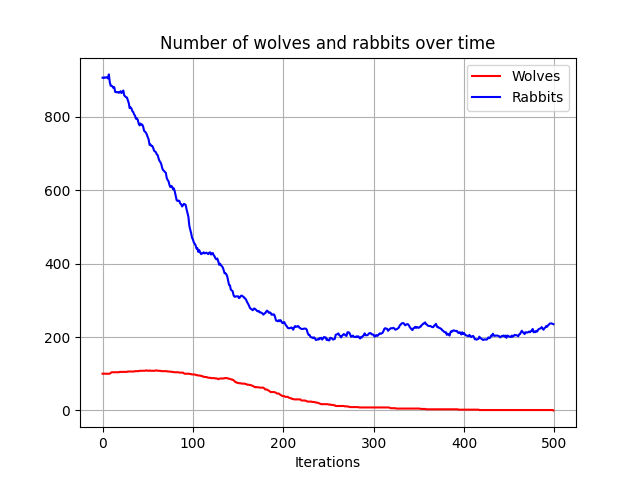
\includegraphics[width=0.5\textwidth]{output_main/PointA.png}
  \caption{PointA;2D; Number of rabbits and wolves over iterations}
\end{figure}
\begin{figure}[H]
  \centering
  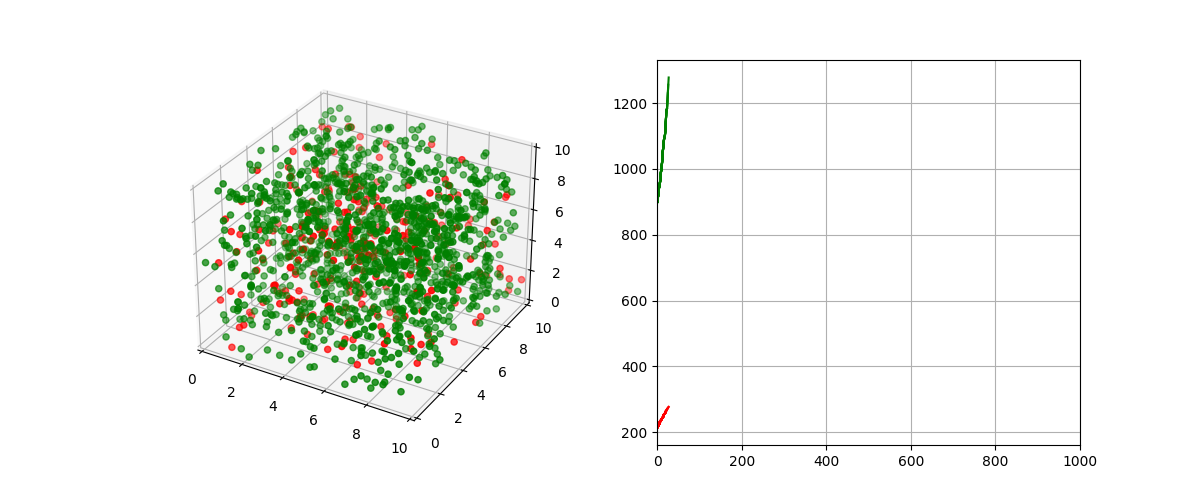
\includegraphics[width=0.6\textwidth]{output3D/3DInitCondition.png}
  \caption{RT visualization}
\end{figure}
In the 3D plot the number of rabbits grows exponentially as well with more than 8000 rabbits only in the very first iterations. 
\begin{figure}[H]
  \centering
  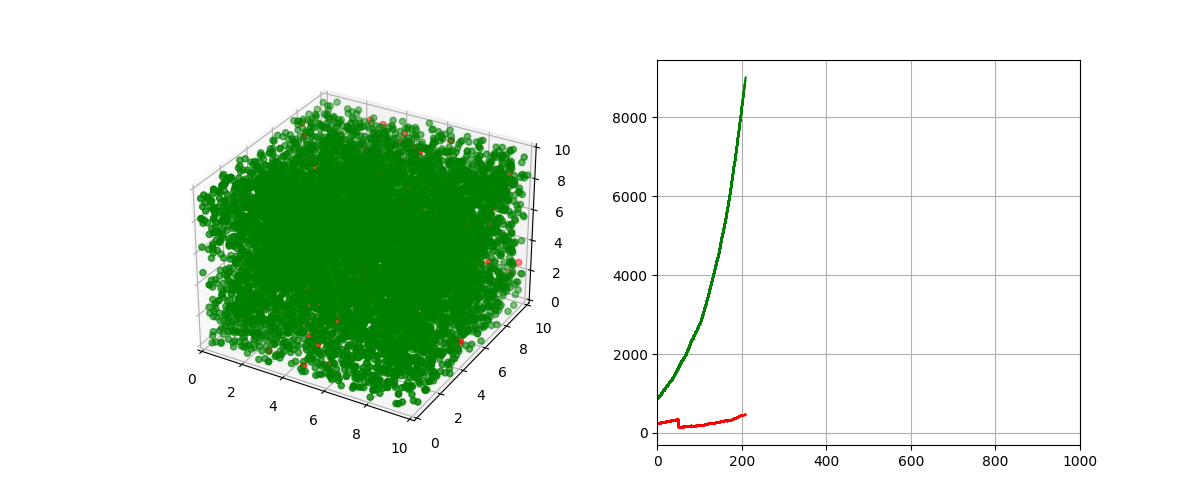
\includegraphics[width=0.6\textwidth]{output3D/secondPlotPointA.png}
  \caption{Environment visualization after just 200 iters} 
\end{figure}
\begin{figure}[H]
  \centering
  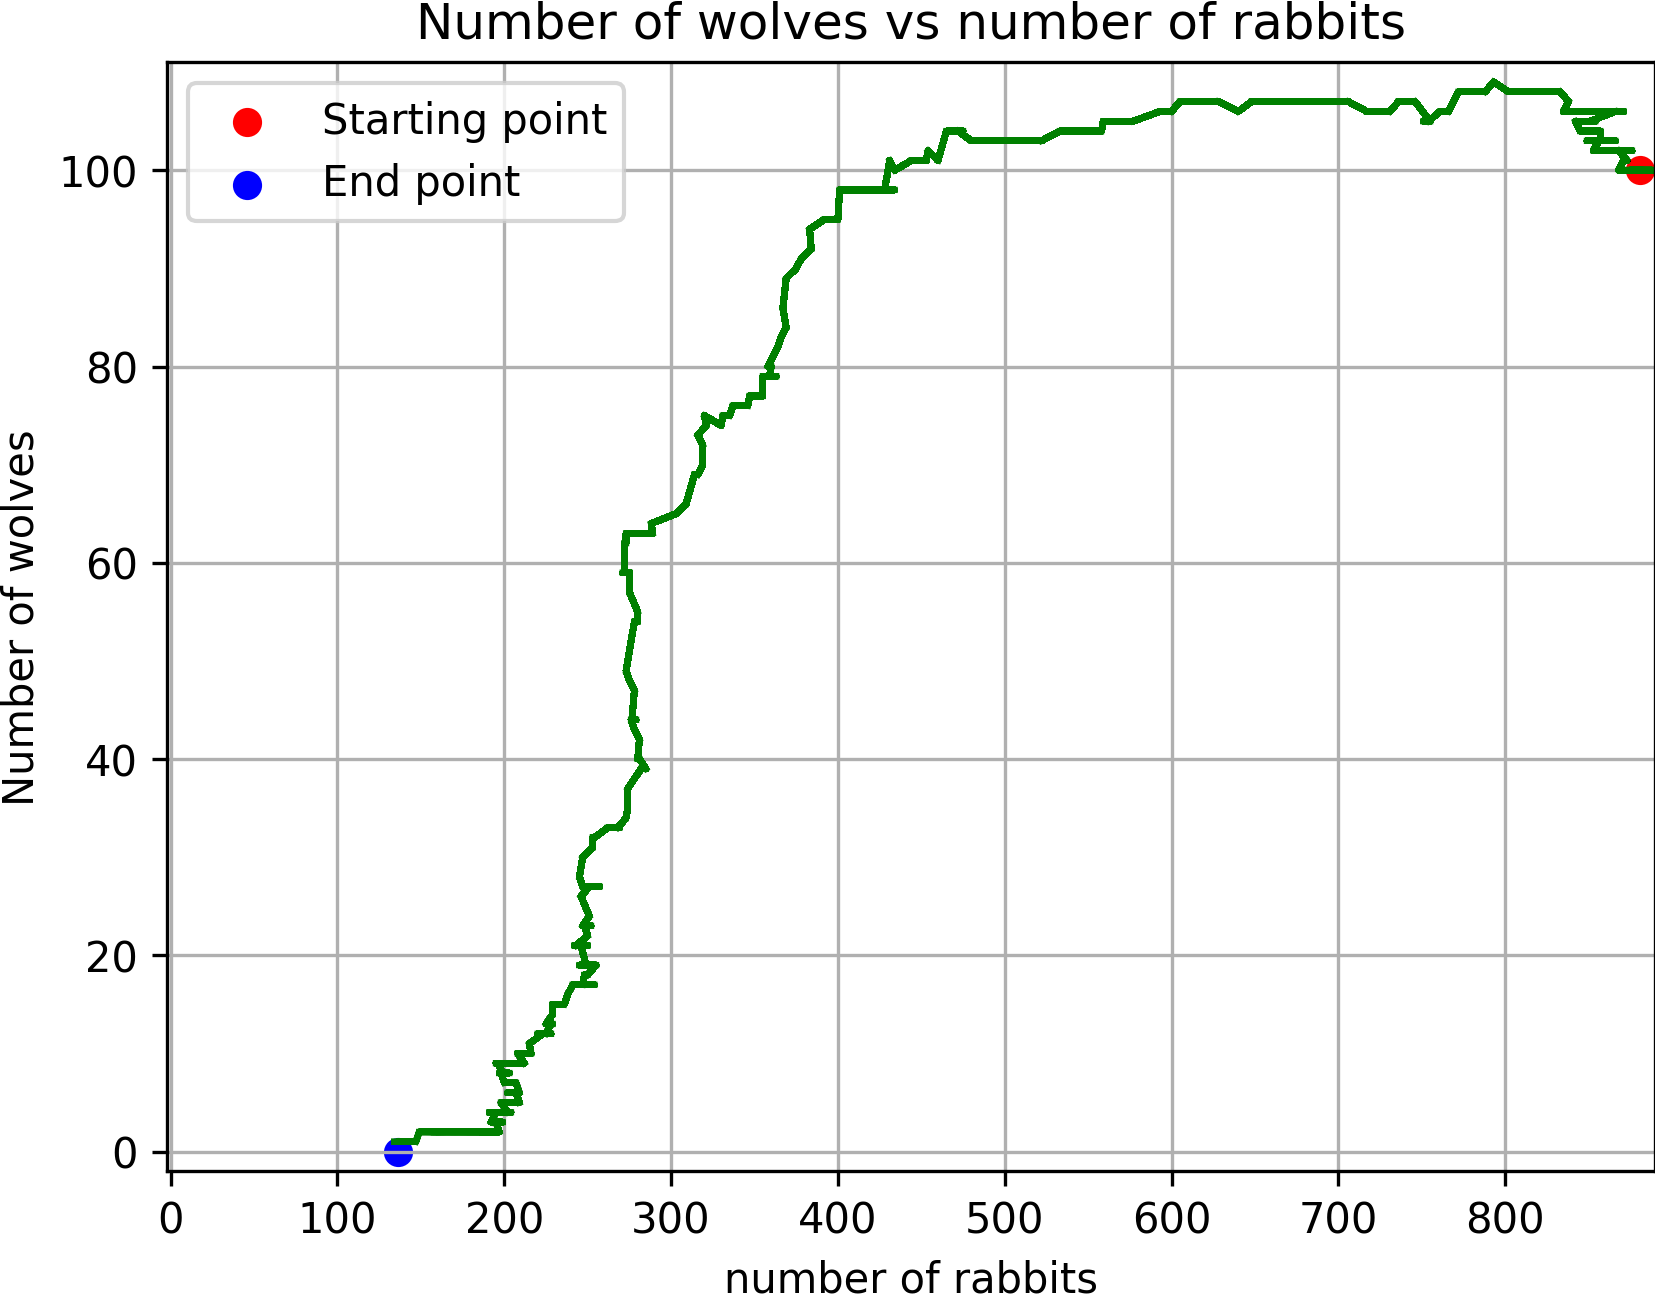
\includegraphics[width=0.6\textwidth]{output_main/PointAnew_populations.png}
  \caption{Population} 
\end{figure}

\section*{Point B}
In this point I set the $t_d^r=50$. However, the situations is even worse than point A because the rabbits live less and no food is provided to the wolves. The number of rabbits and wolves converge very quickly to zero as shown below. 
\begin{figure}[H]
  \centering
  \begin{minipage}[b]{0.435\textwidth}
    \centering
    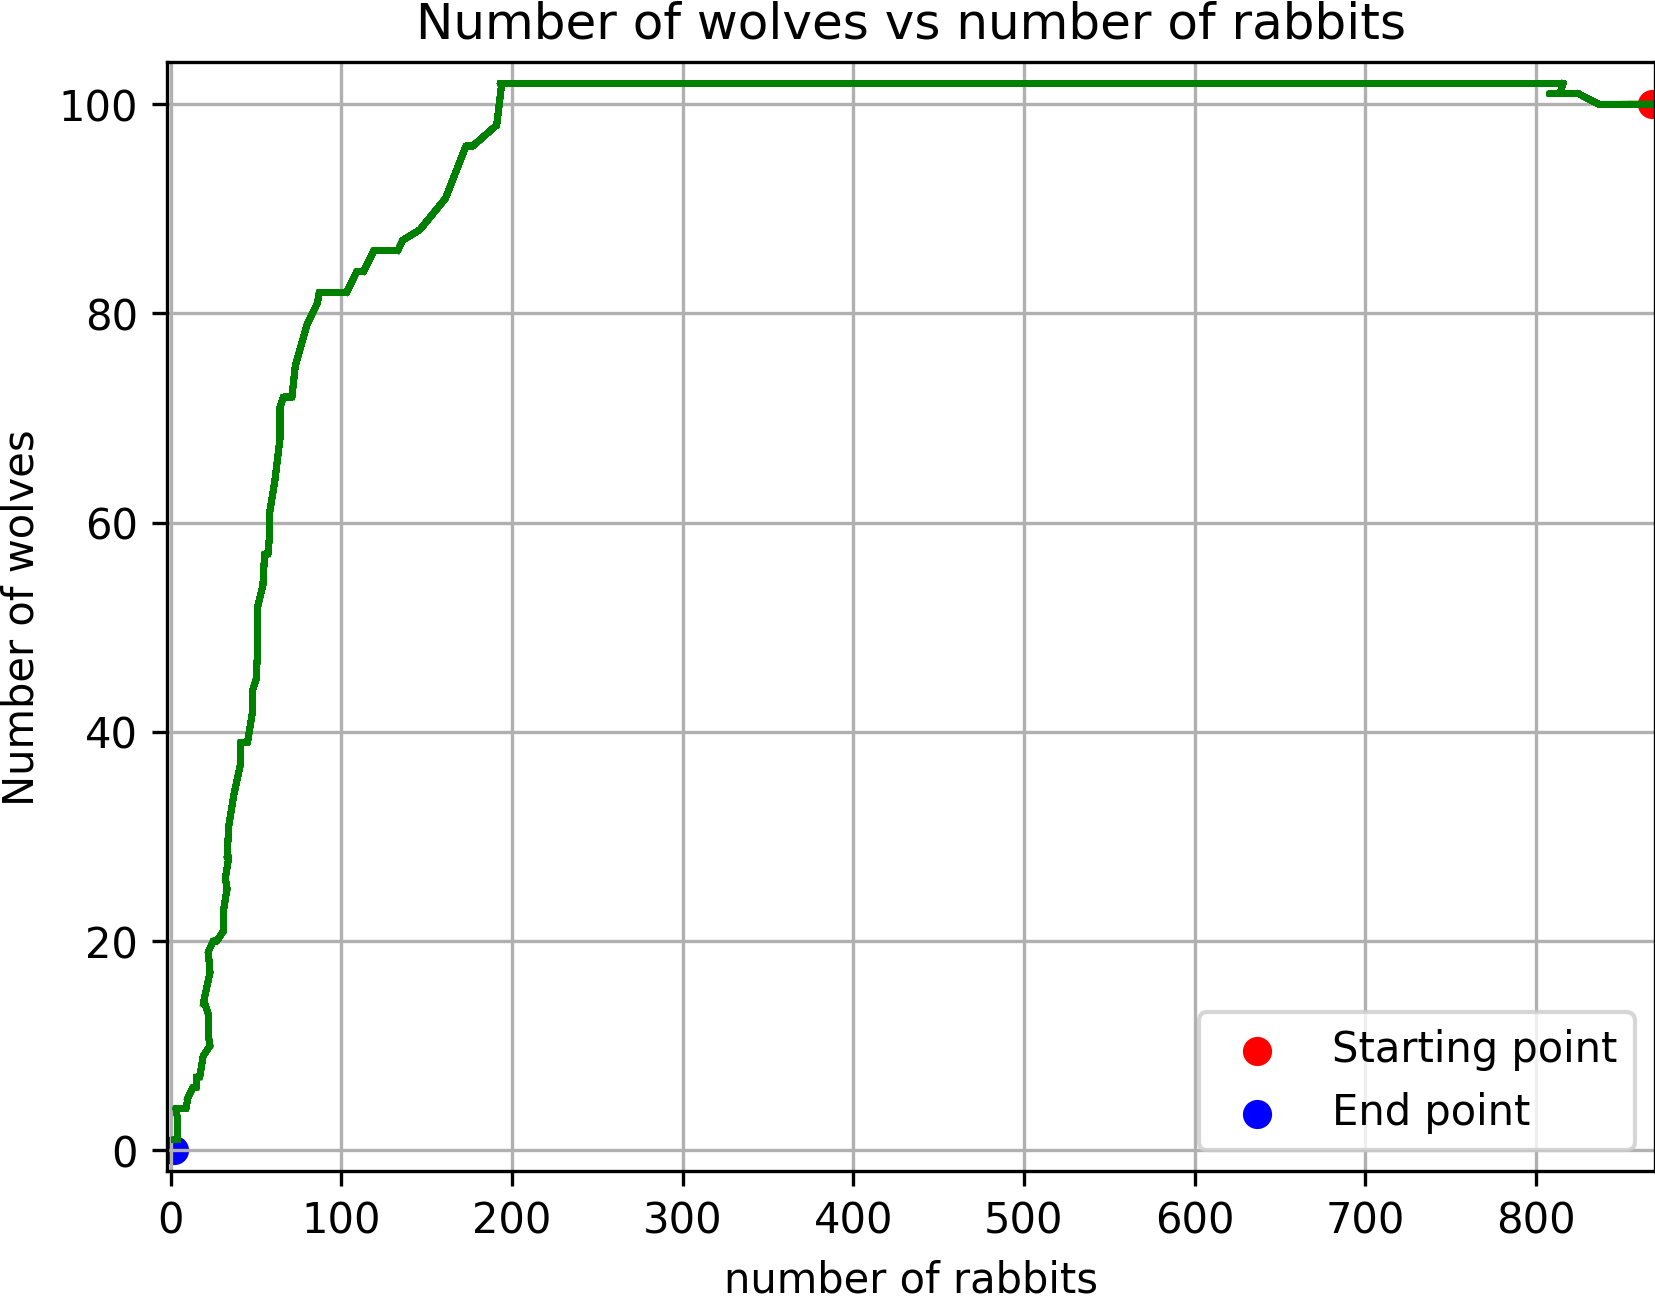
\includegraphics[width=\textwidth]{output_main/PointBnew_populations.png}
    \caption{Population}
  \end{minipage}
  \hfill
  \begin{minipage}[b]{0.49\textwidth}
    \centering
    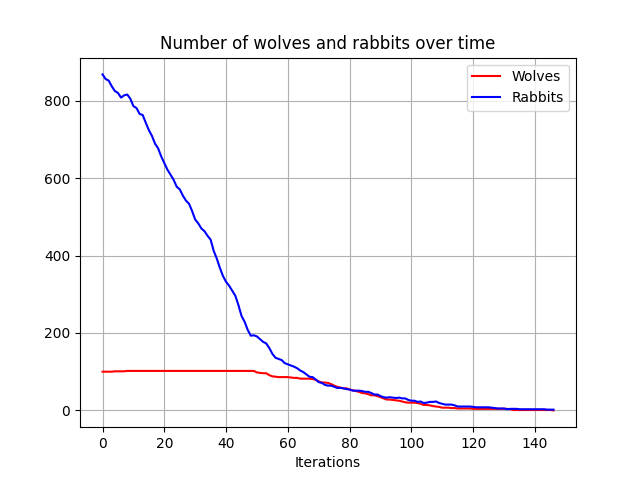
\includegraphics[width=\textwidth]{output_main/PointBnew.png}
    \caption{Population over iterations}
  \end{minipage}
\end{figure}
\section*{Point C}
In this point I set the $\sigma=0.05$. Even with this different parameter the wolves cannot survive more than just 350 iterations probably because the rabbit birth rate is not sufficient. Moreover, the rabbits numbers oscillate every 100 iterations. 
\begin{figure}[H]
  \centering
  \begin{minipage}[b]{0.435\textwidth}
    \centering
    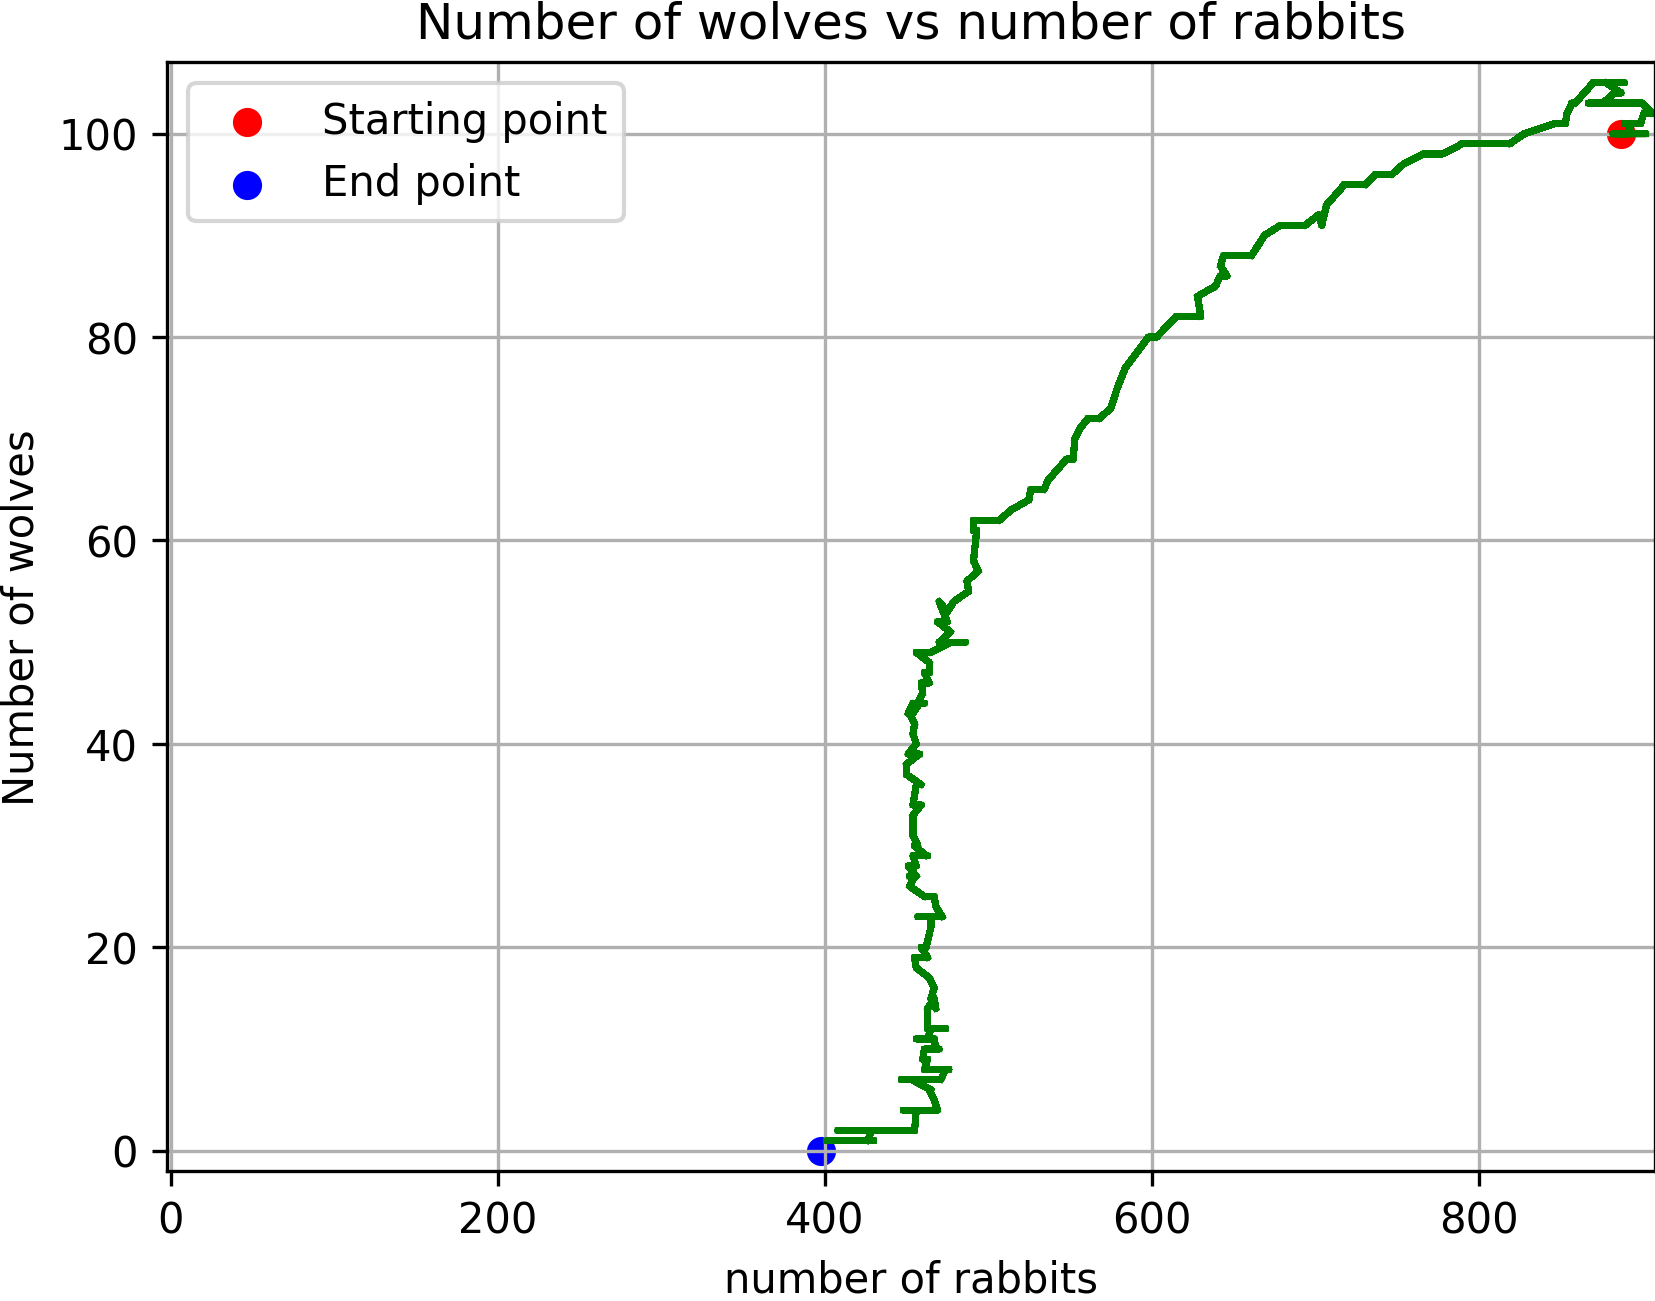
\includegraphics[width=\textwidth]{output_main/PointCnew_populations.png}
    \caption{Population}
  \end{minipage}
  \hfill
  \begin{minipage}[b]{0.49\textwidth}
    \centering
    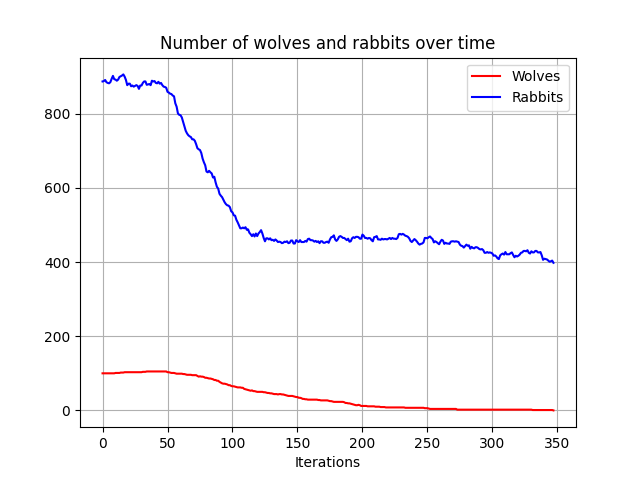
\includegraphics[width=\textwidth]{output_main/PointCnew.png}
    \caption{Population over iterations}
  \end{minipage}
\end{figure}

\section*{My Best parameters}
After many attempts I found optimal paramters for this model. I list what I used:
Note: this are the best only for 2D dimensions. I still have to find out which params are the best for the 3D space. File's name are hardcoded in the python implementations. 
\begin{itemize}
  \item $ITER$: 1000
  \item $N\_R$": 900
  \item $N\_W$: 200, I increase the initial number of wolves
  \item $R\_C$: 0.5
  \item $P\_E_W$: 0.03, I increase the probability of eating a rabbit
  \item $P_R^W$: 0.1, I increase the probability of reproduction rate
  \item $P_R^R$: 0.07 I increase the probability of reproduction rate
  \item $T_D^R$: 100 
  \item $T_D^W$: 50
  \item $ \mu$: 0.0
  \item $\sigma$: 0.05, I used $\sigma$ value of point C
\end{itemize}
I will show 2 runs of this simulation. One with 1000 and $L=10$ and the other with 2000 iterations and $L=8$. 
\subsubsection*{First run, L=10, ITER=1000}
\begin{figure}[H]
  \centering
  \begin{minipage}[b]{0.435\textwidth}
    \centering
    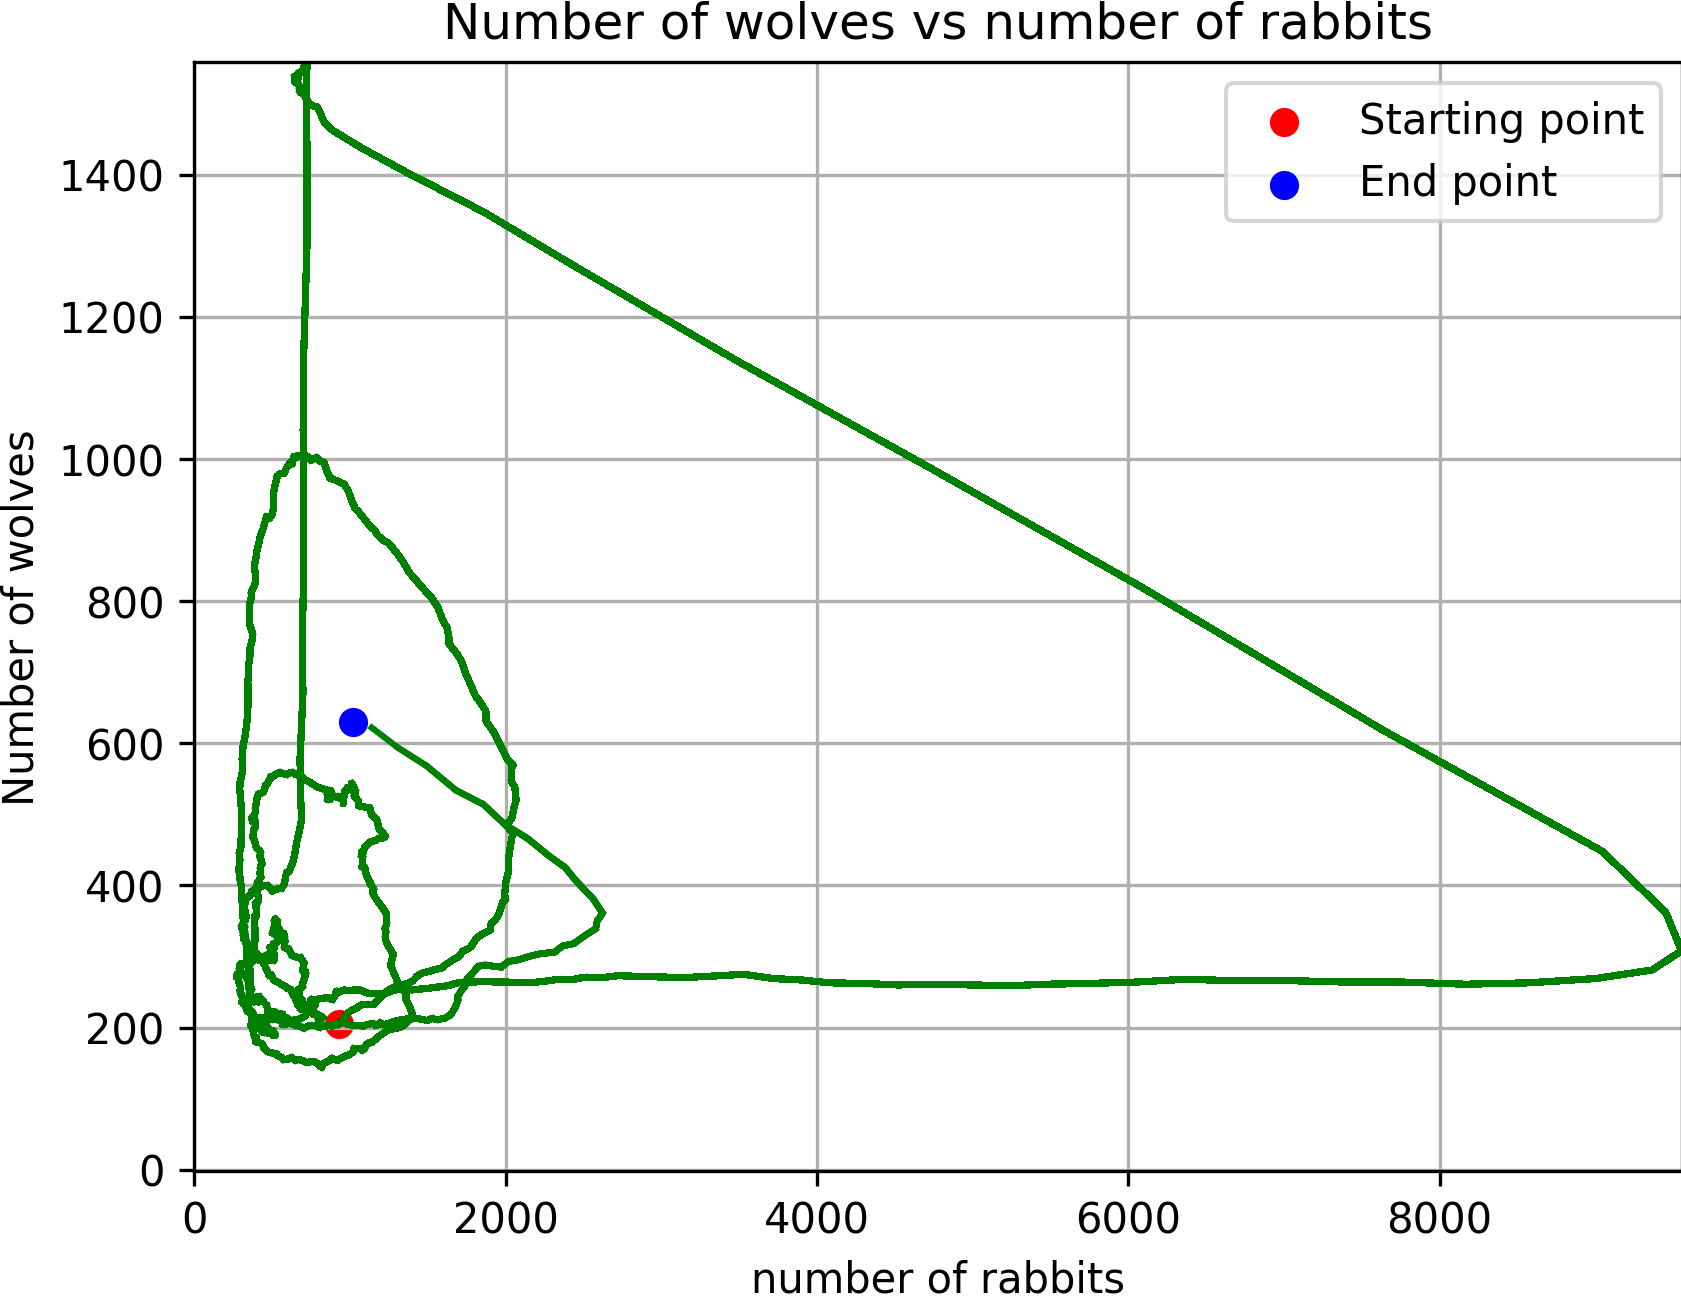
\includegraphics[width=\textwidth]{output_main/Bestnew_populations.png}
    \caption{Population}
  \end{minipage}
  \hfill
  \begin{minipage}[b]{0.49\textwidth}
    \centering
    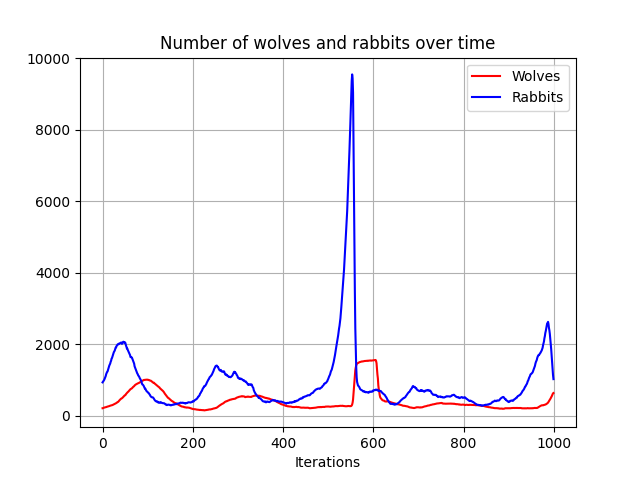
\includegraphics[width=\textwidth]{output_main/Bestnew.png}
    \caption{Population over iterations}
  \end{minipage}
\end{figure}
\subsubsection*{First run, L=8, ITER=2000}
\begin{figure}[H]
  \centering
  \begin{minipage}[b]{0.435\textwidth}
    \centering
    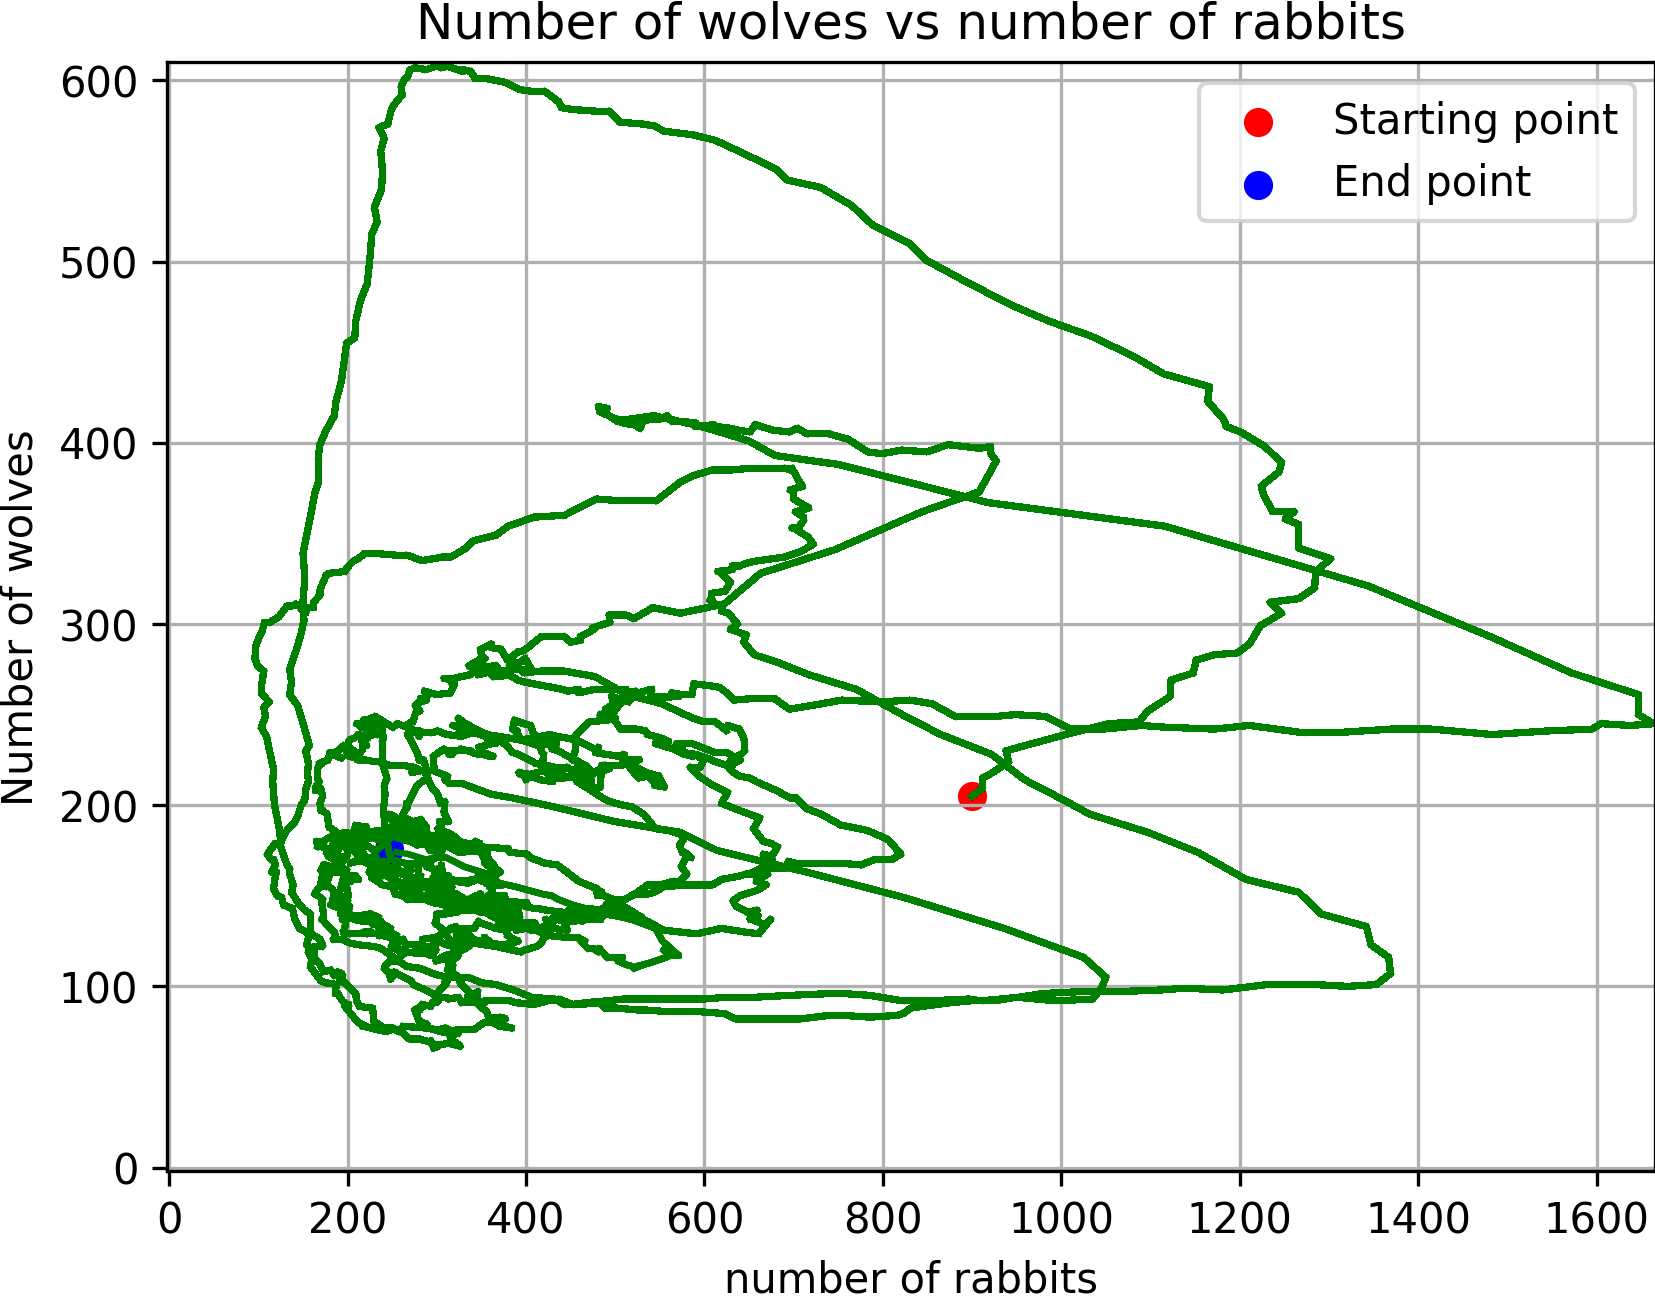
\includegraphics[width=\textwidth]{output_main/Bestnew2_populations.png}
    \caption{Population}
  \end{minipage}
  \hfill
  \begin{minipage}[b]{0.49\textwidth}
    \centering
    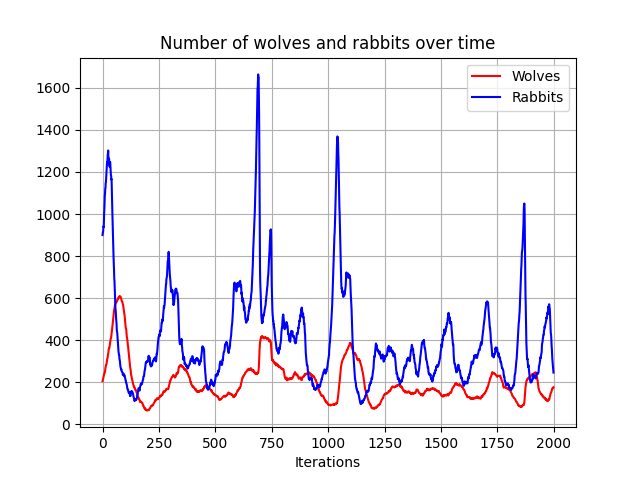
\includegraphics[width=\textwidth]{output_main/Bestnew2.png}
    \caption{Population over iterations}
  \end{minipage}
\end{figure}
\section*{Conclusion}
As one can see these simulations perform much more better than previous points. \\
The plots reflect similarly the beheviour of Lotka–Volterra equations. The parameters used lead to a system equilibria. This is because:\\
\[ y=\alpha/\beta \textit{ and } x= \gamma/\delta\]
where $y=\#wolves$, $x=\#rabbits$, and $\alpha$, $\beta$, $\gamma$, $\delta$ are the parameters of the model.
\end{document}
